\chapter[Marketing do Produto]{Marketing do Produto}

A fim de divulgar o Posicionador de Lente foram desenhados logotipos e construído um site de divulgação. Primeiramente, foi pensado em um nome simples que pudesse caracterizar nosso produto. Utilizando as abreviaturas Po (de Posicionador) e Le (de Lente), formou-se o nome abreviado para o Posicionador de Lente: PoLe. A partir disso, foi realizado o design do logotipo com duas variações, mostradas nas figuras \ref{logo1} e \ref{logo2}. 

O objetivo é utilizar os olhos com uma mira para caracterizar a função do produto: posicionar lentes de contato. Os traços e as cores escolhidas tanto para o logotipo quanto para o site passam a ideia de algo delicado e limpo.

\begin{figure}[H]
		\centering
			
\includegraphics[scale=0.5, angle=90]{figuras/logo1.png}
		\caption{Logotipo 1}
		\label{logo1}
\end{figure}

\begin{figure}[H]
		\centering
			
\includegraphics[scale=1.0]{figuras/logo2.png}
		\caption{Logotipo 2}
		\label{logo2}
\end{figure}


O site de divulgação do produto é apresentado na figura \ref{site1}.

\begin{figure}[H]
		\centering
			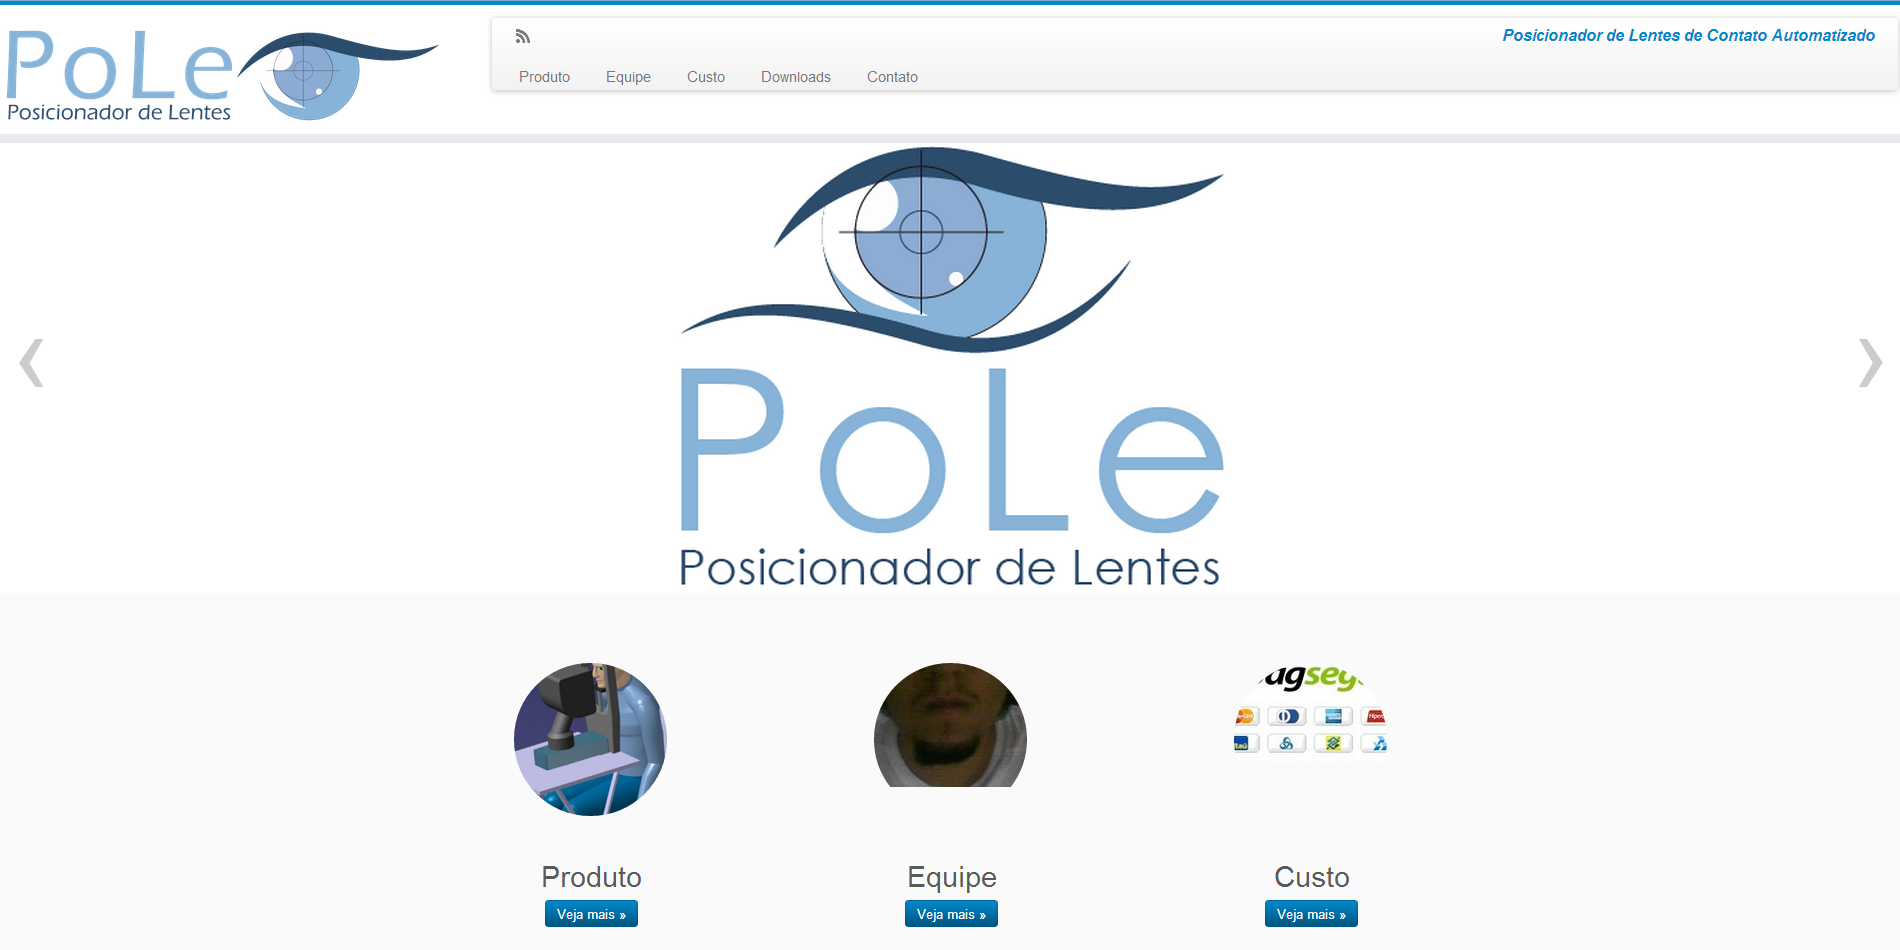
\includegraphics[scale=0.3]{figuras/site1.png}
		\caption{Home do Site}
		\label{site1}
\end{figure}

A ideia é que por meio do site, os clientes possam conhecer um pouco mais sobre o produto, sobre a equipe que o desenvolveu e o custo do produto. Além de poder realizar a encomenda do produto e entrar em contato com os desenvolvedores. Também estará disponível no site a documentação do produto, que consiste neste relatório, e links de artigos úteis relacionados ao uso de lentes de contato.

\begin{figure}[H]
		\centering
			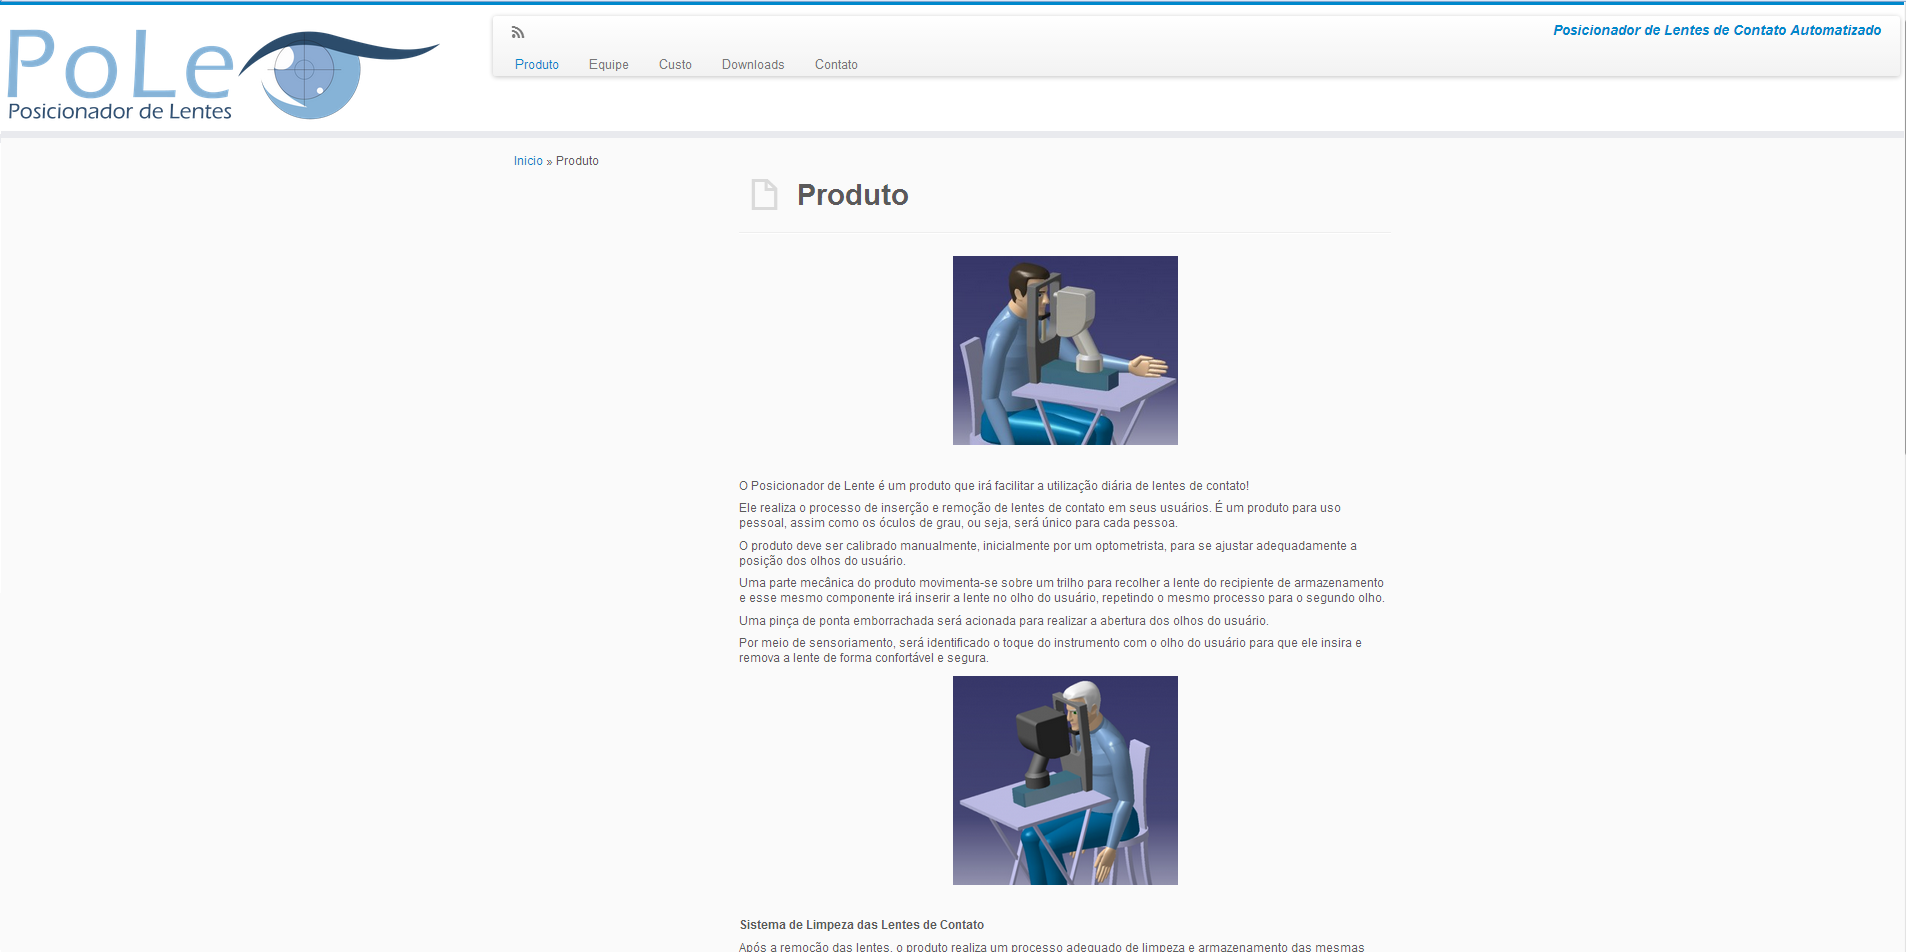
\includegraphics[scale=0.3]{figuras/site5.png}
		\caption{Página sobre o Produto}
		\label{site5}
\end{figure}


\begin{figure}[H]
		\centering
			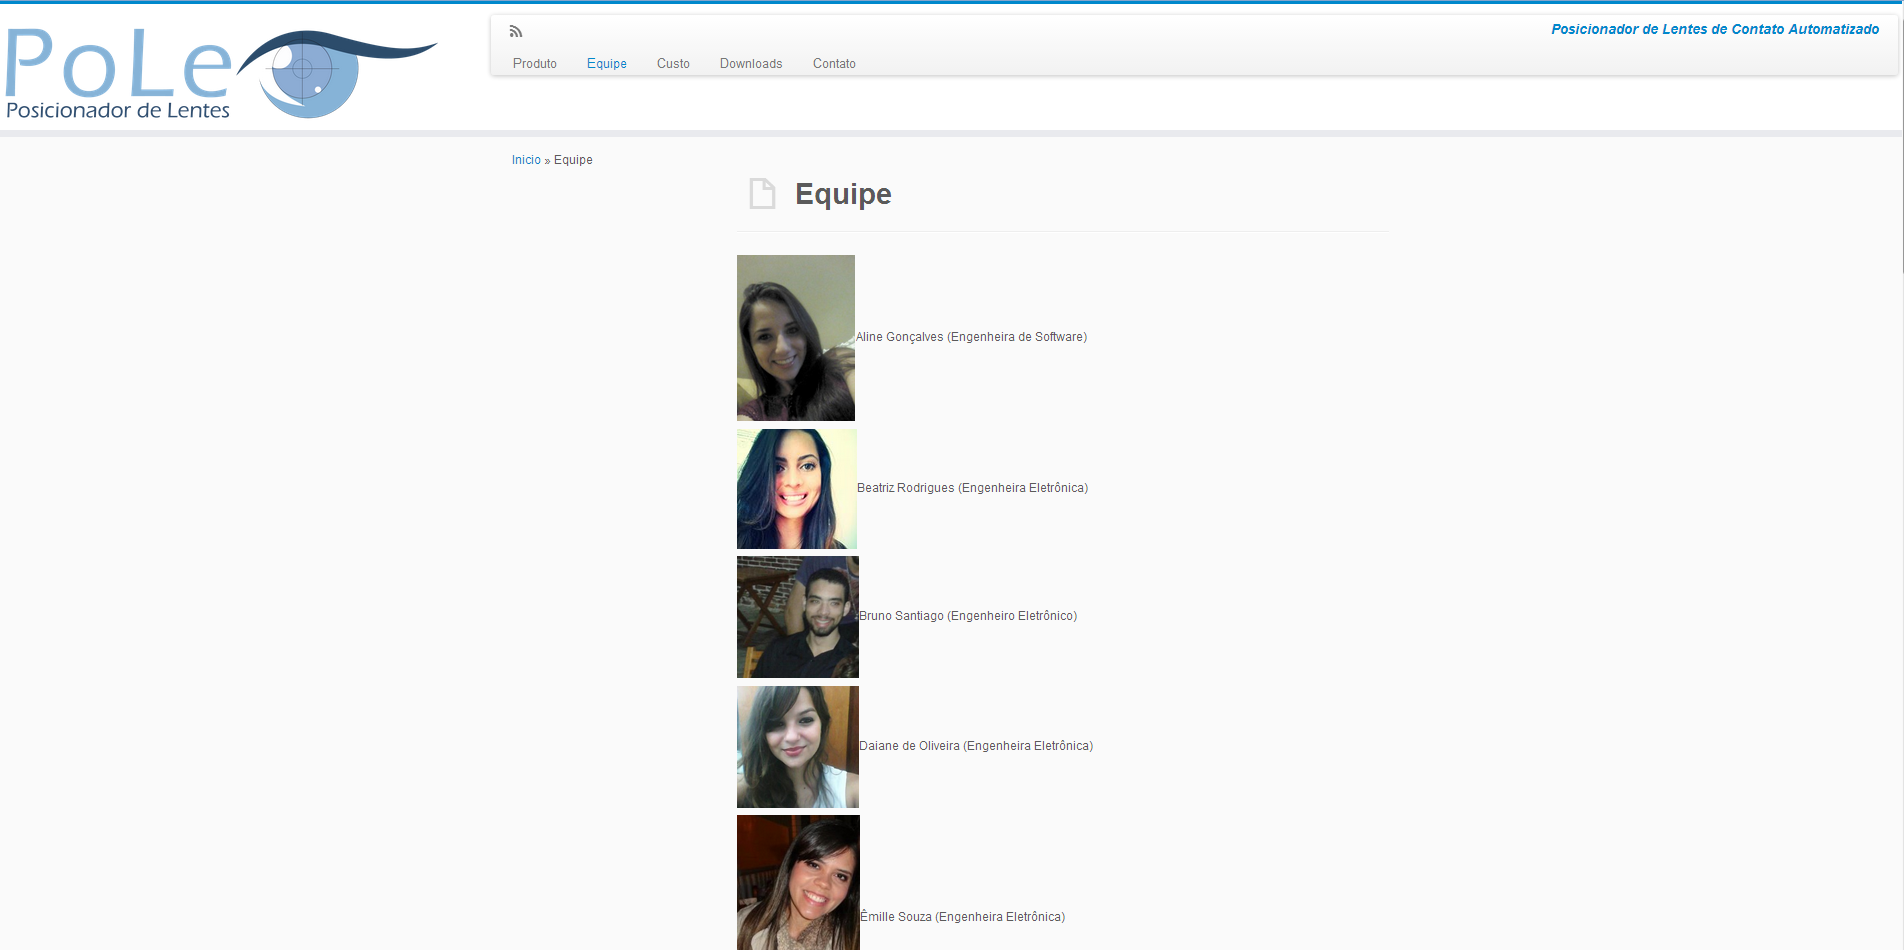
\includegraphics[scale=0.3]{figuras/site4.png}
		\caption{Página da Equipe}
		\label{site4}
\end{figure}


\begin{figure}[H]
		\centering
			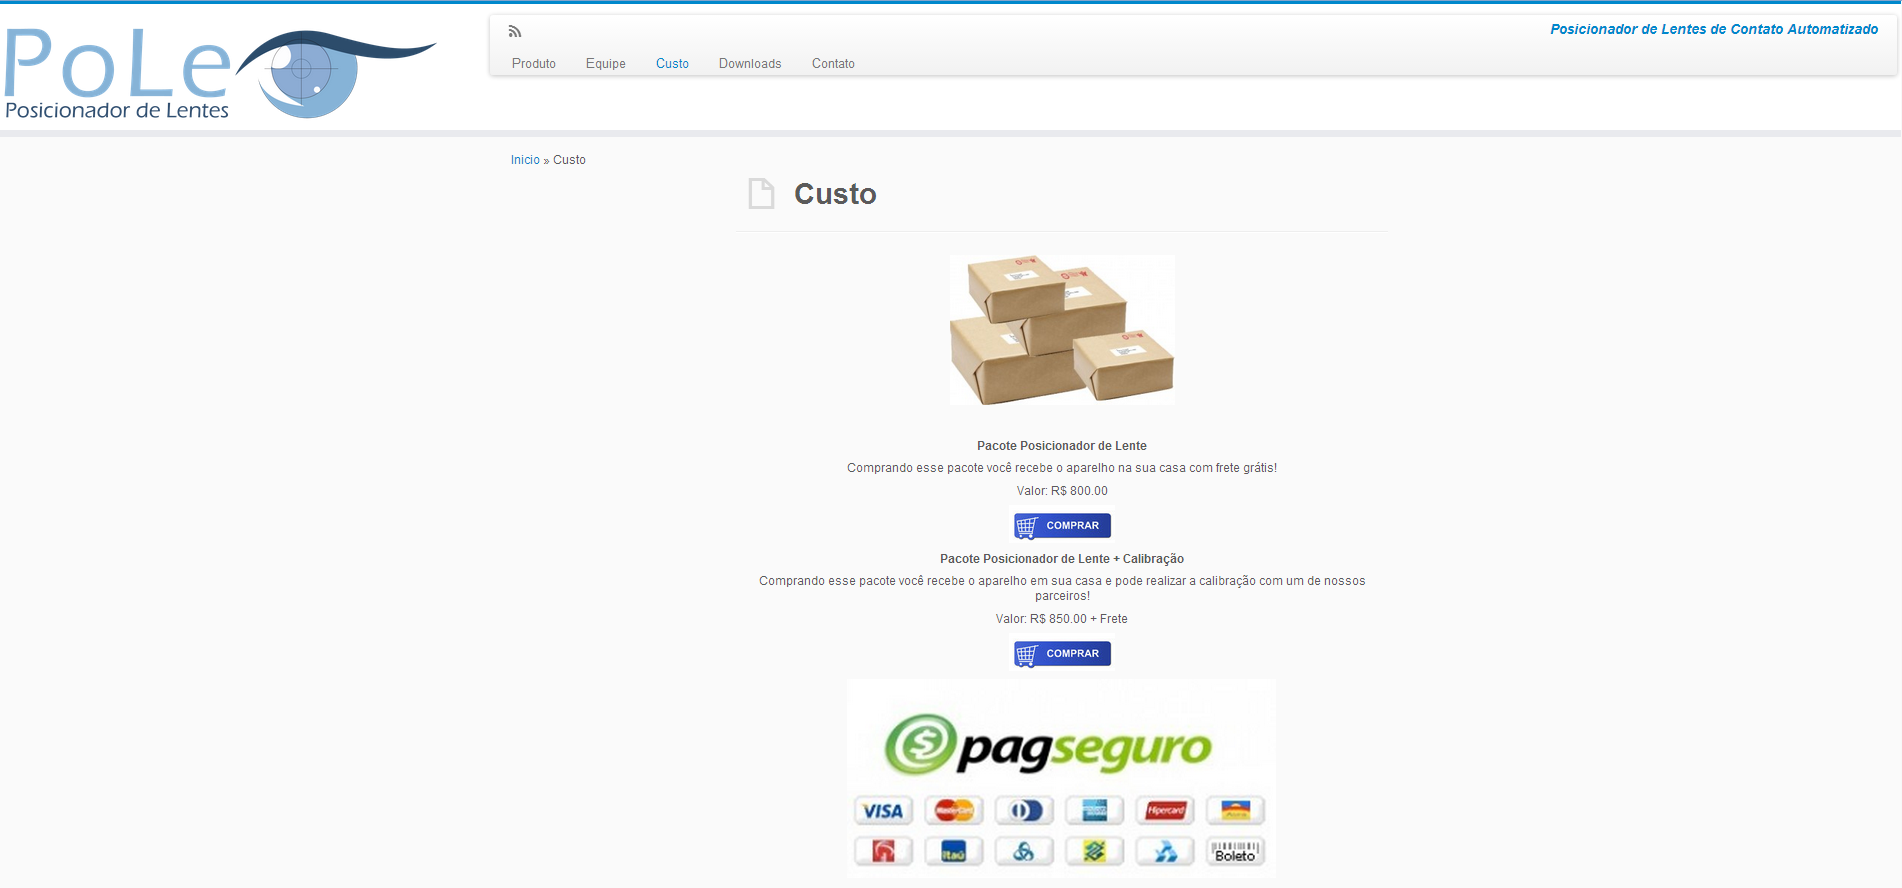
\includegraphics[scale=0.3]{figuras/site2.png}
		\caption{Página de Compra}
		\label{site2}
\end{figure}


\begin{figure}[H]
		\centering
			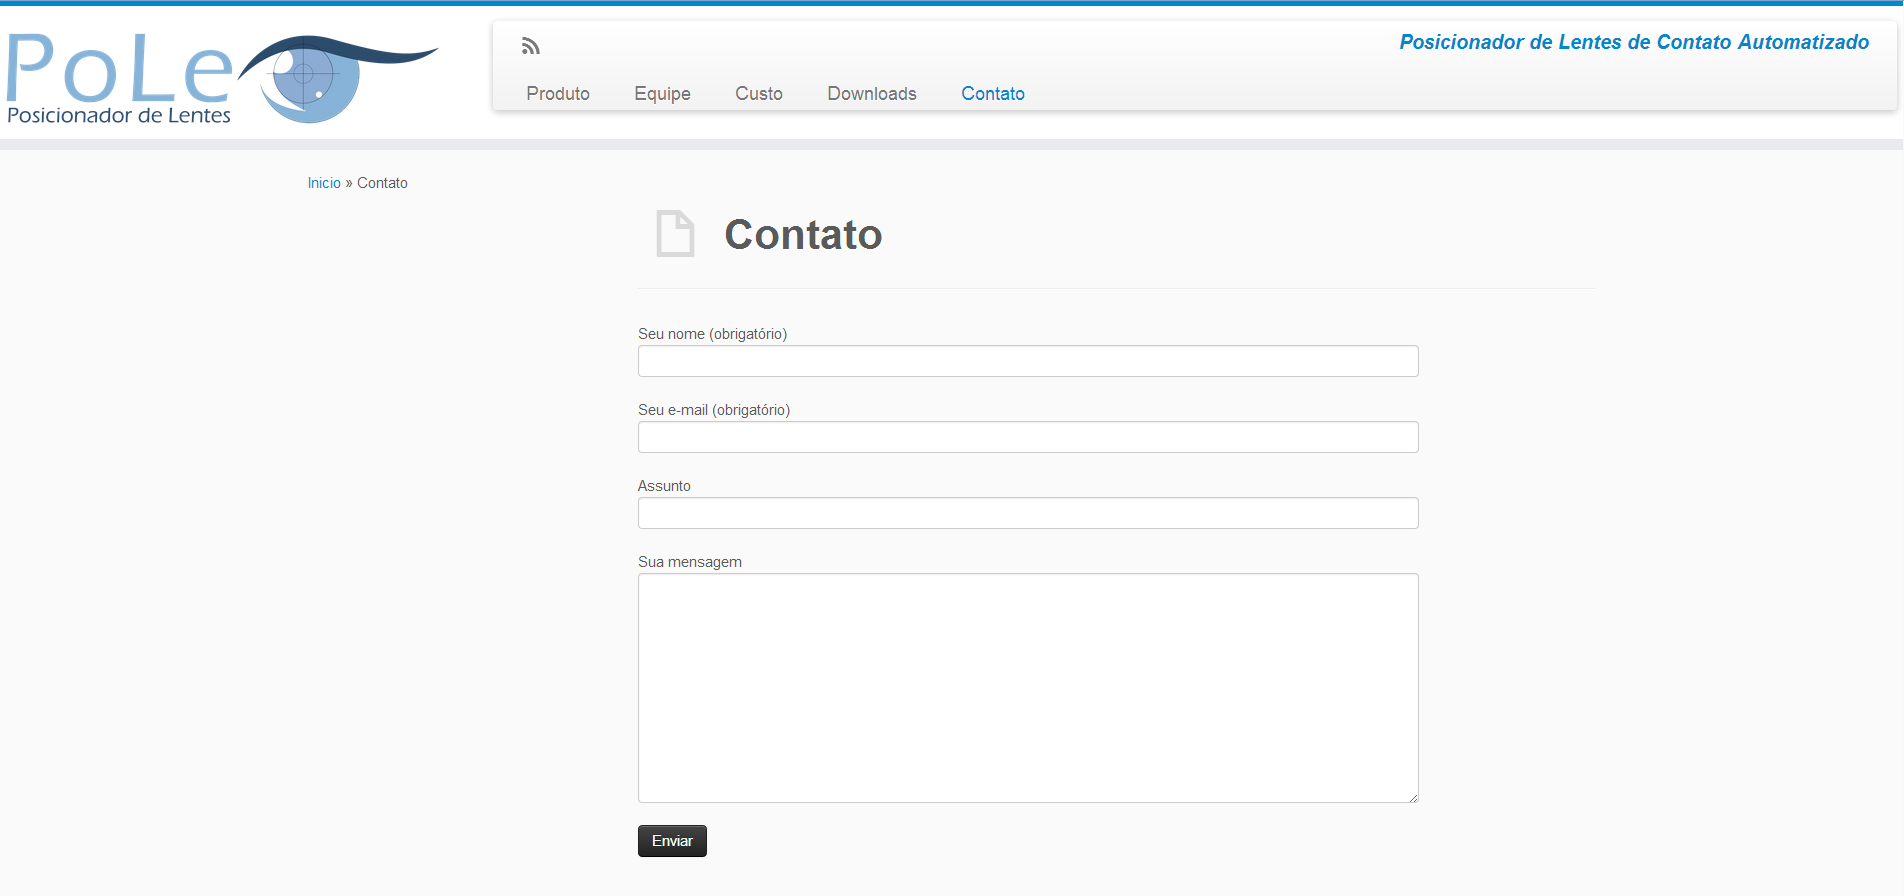
\includegraphics[scale=0.3]{figuras/site3.png}
		\caption{Página de Contato}
		\label{site3}
\end{figure}


Para criação do site utilizou-se o WordPress, que é um aplicativo para gerenciamento de conteúdo para web, implementado em linguagem PHP com banco de dados MySql. É amplamente utilizado para criação de sites dos tipos blogs. Seu uso é intensificado principalmente por ser de código aberto. Sua licença é distribuída pela GNU General Public License.
	
Dentre as atividades comuns permitidas pelo WordPress estão as seguintes:
 
\begin{itemize}
\item Criação de posts;
\item Criação de páginas;
\item Uso de imagens e vídeos;
\item Galeria de imagens;
\item Criação de painéis;
\item Widgets em temas;
\item Gerenciamento de comentários;
\item Smiles e Emoticons; e
\item Cabeçalhos personalizados.
\end{itemize} 

O WordPress foi projetado para ser instalado no seu próprio servidor web ou conta de hospedagem compartilhada, o que dá ao proprietário do site controle completo. Além disso, é possível realizar um gerenciamento de usuários, o que permite controlar o acesso dos usuários a diferentes recursos.
	
Para construção do site de divulgação do posicionador de lentes, além do WordPress, foi utilizada a arquitetura definida pelo WampServer, que permite criar aplicações web com Apache2, PHP e um banco de dados MySql, que pode ser gerenciado pelo phpMyAdmin. A Figura \ref{arquitetura} apresenta a arquitetura utilizada para construção do site de divulgação.


\begin{figure}[H]
		\centering
			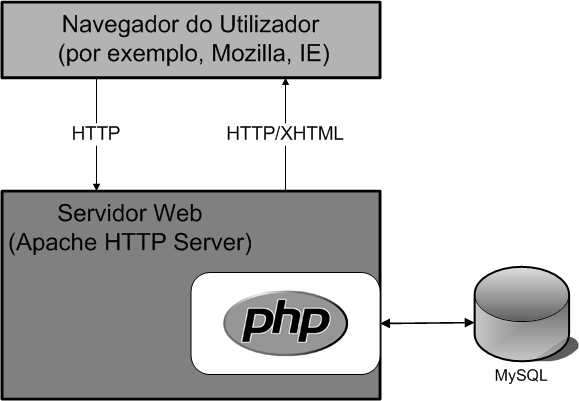
\includegraphics[scale=1.0]{figuras/arquitetura.png}
		\caption{Arquitetura WAMP (Windows, Apache, MySql e PHP)}
		\label{arquitetura}
\end{figure}

Conforme a figura \ref{arquitetura}, o funcionamento do sistema que utiliza a arquitetura WAMP baseia-se no modelo cliente-servidor, sobre um protocolo de rede HTTP. Neste caso, o utilizador requisita um determinado ficheiro constante em um computador remoto, passando um endereço de URL. Normalmente o pedido é efetuado por um navegador WEB. Após o servidor remoto compreender a requisição do utilizador, o ficheiro será devolvido.
	
Com a arquitetura WAMP e com o uso do WordPress será possível atingir os objetivos do site de divulgação do posicionador de lentes, que se resumem em apresentar o funcionamento do produto, a equipe responsável por sua confecção e seus custos.



